

\documentclass[svgnames,addpoints]{exam}



\usepackage[T1]{fontenc}
\usepackage[utf8]{inputenc}
\usepackage[spanish]{babel}

\usepackage{tb}

\usepackage{amsfonts}
\usepackage{amssymb}
\usepackage{mathtools}

\usepackage{pifont}

\usepackage{cancel}
\usepackage{array}

\usepackage{tikz}
\usepackage{pgflibraryarrows}
\usepackage{pgflibrarysnakes}

\usetikzlibrary{matrix,patterns,fadings,positioning}

\usepackage{array}
\usepackage{eurosym}

\usepackage{booktabs}
\usepackage{url}

\usepackage{rotating}



\begin{document}

\titulacion{Colegio Tomás Bretón}
\asignatura{ 1º A }

\convocatoria{\today}
\tiempo{4 horas}

\begin{tabular}{cc}

  \begin{minipage}{7.5cm}

    \begin{tabular}{c}

      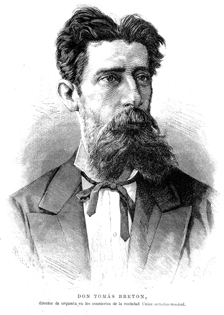
\includegraphics[scale=0.4]{tomas-breton}\\

    \end{tabular}

  \end{minipage}
  &
  \begin{minipage}{8.5cm}

    \begin{center}

      {\huge \bf \titu}\\
      {\Large \bf \asig}\\ \ \\
      
      \convo

    \end{center}

  \end{minipage}\\ & \\ & \\  & \\

\end{tabular}

\vspace*{-0.5cm}

\begin{tikzpicture}[remember picture, overlay]
  \node[xshift=-.5cm,yshift=1.8cm,opacity=0.4,inner sep=0pt] at (current page.center) {
    
\includegraphics[width=18.0cm, height=12.0cm]{images/Pergamino}
  };
\end{tikzpicture}  

\begin{center}
  
    \begin{minipage}{13cm}
      \vspace*{0.3cm}
      
      Carta del Ministerio de la Maravilla y la Inteligencia para Adriana\\
      
      Querida alumna del Tomás Bretón:\\[0.2cm]
	
      \vspace*{-0.25cm}
      \begin{tabular}{c}
        
        \begin{minipage}{12cm}

        Probablemente no habrás oído hablar de nuestro ministerio, eso es porque es un ministerio secreto. Sólo nos ponemos en contacto con la gente que es tan lista y maravillosa que tiene que formar parte de él. \\
	
        Tus profesores Jorge y Paloma nos han dicho las buenas notas que has sacado en esta evaluación. Las notas han sido las mejores de todo el país, pero necesitamos saber si son verdad o no. Por eso hemos hecho estas actividades para que las hagas si quieres demostrar que eres de las alumnas más listas y maravillosas de toda España. ?`Te atreves a realizarlas? Si tienes alguna duda puedes preguntarle a papá o a mamá.\\

        !`Mucha suerte!\\
	
        \end{minipage}
        
      \end{tabular}
      
    \end{minipage}

\end{center}

\vspace*{2.0cm}



{\Large\bf Sumas}

El primer paso para demostrar que eres de las más listas
será hacer estas sumas. Como ves son muy facilitas, sólo es el
calentamiento:

\noindent\begin{minipage}{0.25\linewidth}  
  \begin{center}
    \begin{tikzpicture}

      % draw an invisible box used to properly align all sequences
      \draw [white] (0,0) rectangle (3.5,4.0);

      % show the operands
      \node (label1) at (2.5, 3.5) {};
      \node [left=0.0 cm of label1] (num1) {\huge 2};
      \node (label2) at (2.5, 2.5) {};
      \node [left=0.0 cm of label2] (num2) {\huge 3};

      % show a straight line
      \draw [thick] (0.5, 2.0) -- (3.0, 2.0);

      % show the operator
      \node (op) at (1, 2.5) {\huge$+$};

      % show the result
      \node (label3) at (2.75, 1) {};
      \node [rounded corners, rectangle, minimum width=1.5 cm, minimum height = 1.25 cm, draw, left=0.0 cm of label3] {};

    \end{tikzpicture}
  \end{center}
\end{minipage}
\begin{minipage}{0.25\linewidth}  
  \begin{center}
    \begin{tikzpicture}

      % draw an invisible box used to properly align all sequences
      \draw [white] (0,0) rectangle (3.5,4.0);

      % show the operands
      \node (label1) at (2.5, 3.5) {};
      \node [left=0.0 cm of label1] (num1) {\huge 9};
      \node (label2) at (2.5, 2.5) {};
      \node [left=0.0 cm of label2] (num2) {\huge 6};

      % show a straight line
      \draw [thick] (0.5, 2.0) -- (3.0, 2.0);

      % show the operator
      \node (op) at (1, 2.5) {\huge$+$};

      % show the result
      \node (label3) at (2.75, 1) {};
      \node [rounded corners, rectangle, minimum width=1.5 cm, minimum height = 1.25 cm, draw, left=0.0 cm of label3] {};

    \end{tikzpicture}
  \end{center}
\end{minipage}
\begin{minipage}{0.25\linewidth}  
  \begin{center}
    \begin{tikzpicture}

      % draw an invisible box used to properly align all sequences
      \draw [white] (0,0) rectangle (3.5,4.0);

      % show the operands
      \node (label1) at (2.5, 3.5) {};
      \node [left=0.0 cm of label1] (num1) {\huge 4};
      \node (label2) at (2.5, 2.5) {};
      \node [left=0.0 cm of label2] (num2) {\huge 3};

      % show a straight line
      \draw [thick] (0.5, 2.0) -- (3.0, 2.0);

      % show the operator
      \node (op) at (1, 2.5) {\huge$+$};

      % show the result
      \node (label3) at (2.75, 1) {};
      \node [rounded corners, rectangle, minimum width=1.5 cm, minimum height = 1.25 cm, draw, left=0.0 cm of label3] {};

    \end{tikzpicture}
  \end{center}
\end{minipage}
\begin{minipage}{0.25\linewidth}  
  \begin{center}
    \begin{tikzpicture}

      % draw an invisible box used to properly align all sequences
      \draw [white] (0,0) rectangle (3.5,4.0);

      % show the operands
      \node (label1) at (2.5, 3.5) {};
      \node [left=0.0 cm of label1] (num1) {\huge 5};
      \node (label2) at (2.5, 2.5) {};
      \node [left=0.0 cm of label2] (num2) {\huge 5};

      % show a straight line
      \draw [thick] (0.5, 2.0) -- (3.0, 2.0);

      % show the operator
      \node (op) at (1, 2.5) {\huge$+$};

      % show the result
      \node (label3) at (2.75, 1) {};
      \node [rounded corners, rectangle, minimum width=1.5 cm, minimum height = 1.25 cm, draw, left=0.0 cm of label3] {};

    \end{tikzpicture}
  \end{center}
\end{minipage}
\begin{minipage}{0.25\linewidth}  
  \begin{center}
    \begin{tikzpicture}

      % draw an invisible box used to properly align all sequences
      \draw [white] (0,0) rectangle (3.5,4.0);

      % show the operands
      \node (label1) at (2.5, 3.5) {};
      \node [left=0.0 cm of label1] (num1) {\huge 7};
      \node (label2) at (2.5, 2.5) {};
      \node [left=0.0 cm of label2] (num2) {\huge 5};

      % show a straight line
      \draw [thick] (0.5, 2.0) -- (3.0, 2.0);

      % show the operator
      \node (op) at (1, 2.5) {\huge$+$};

      % show the result
      \node (label3) at (2.75, 1) {};
      \node [rounded corners, rectangle, minimum width=1.5 cm, minimum height = 1.25 cm, draw, left=0.0 cm of label3] {};

    \end{tikzpicture}
  \end{center}
\end{minipage}
\begin{minipage}{0.25\linewidth}  
  \begin{center}
    \begin{tikzpicture}

      % draw an invisible box used to properly align all sequences
      \draw [white] (0,0) rectangle (3.5,4.0);

      % show the operands
      \node (label1) at (2.5, 3.5) {};
      \node [left=0.0 cm of label1] (num1) {\huge 8};
      \node (label2) at (2.5, 2.5) {};
      \node [left=0.0 cm of label2] (num2) {\huge 1};

      % show a straight line
      \draw [thick] (0.5, 2.0) -- (3.0, 2.0);

      % show the operator
      \node (op) at (1, 2.5) {\huge$+$};

      % show the result
      \node (label3) at (2.75, 1) {};
      \node [rounded corners, rectangle, minimum width=1.5 cm, minimum height = 1.25 cm, draw, left=0.0 cm of label3] {};

    \end{tikzpicture}
  \end{center}
\end{minipage}
\begin{minipage}{0.25\linewidth}  
  \begin{center}
    \begin{tikzpicture}

      % draw an invisible box used to properly align all sequences
      \draw [white] (0,0) rectangle (3.5,4.0);

      % show the operands
      \node (label1) at (2.5, 3.5) {};
      \node [left=0.0 cm of label1] (num1) {\huge 3};
      \node (label2) at (2.5, 2.5) {};
      \node [left=0.0 cm of label2] (num2) {\huge 2};

      % show a straight line
      \draw [thick] (0.5, 2.0) -- (3.0, 2.0);

      % show the operator
      \node (op) at (1, 2.5) {\huge$+$};

      % show the result
      \node (label3) at (2.75, 1) {};
      \node [rounded corners, rectangle, minimum width=1.5 cm, minimum height = 1.25 cm, draw, left=0.0 cm of label3] {};

    \end{tikzpicture}
  \end{center}
\end{minipage}
\begin{minipage}{0.25\linewidth}  
  \begin{center}
    \begin{tikzpicture}

      % draw an invisible box used to properly align all sequences
      \draw [white] (0,0) rectangle (3.5,4.0);

      % show the operands
      \node (label1) at (2.5, 3.5) {};
      \node [left=0.0 cm of label1] (num1) {\huge 9};
      \node (label2) at (2.5, 2.5) {};
      \node [left=0.0 cm of label2] (num2) {\huge 9};

      % show a straight line
      \draw [thick] (0.5, 2.0) -- (3.0, 2.0);

      % show the operator
      \node (op) at (1, 2.5) {\huge$+$};

      % show the result
      \node (label3) at (2.75, 1) {};
      \node [rounded corners, rectangle, minimum width=1.5 cm, minimum height = 1.25 cm, draw, left=0.0 cm of label3] {};

    \end{tikzpicture}
  \end{center}
\end{minipage}
\begin{minipage}{0.25\linewidth}  
  \begin{center}
    \begin{tikzpicture}

      % draw an invisible box used to properly align all sequences
      \draw [white] (0,0) rectangle (3.5,4.0);

      % show the operands
      \node (label1) at (2.5, 3.5) {};
      \node [left=0.0 cm of label1] (num1) {\huge 7};
      \node (label2) at (2.5, 2.5) {};
      \node [left=0.0 cm of label2] (num2) {\huge 1};

      % show a straight line
      \draw [thick] (0.5, 2.0) -- (3.0, 2.0);

      % show the operator
      \node (op) at (1, 2.5) {\huge$+$};

      % show the result
      \node (label3) at (2.75, 1) {};
      \node [rounded corners, rectangle, minimum width=1.5 cm, minimum height = 1.25 cm, draw, left=0.0 cm of label3] {};

    \end{tikzpicture}
  \end{center}
\end{minipage}
\begin{minipage}{0.25\linewidth}  
  \begin{center}
    \begin{tikzpicture}

      % draw an invisible box used to properly align all sequences
      \draw [white] (0,0) rectangle (3.5,4.0);

      % show the operands
      \node (label1) at (2.5, 3.5) {};
      \node [left=0.0 cm of label1] (num1) {\huge 3};
      \node (label2) at (2.5, 2.5) {};
      \node [left=0.0 cm of label2] (num2) {\huge 1};

      % show a straight line
      \draw [thick] (0.5, 2.0) -- (3.0, 2.0);

      % show the operator
      \node (op) at (1, 2.5) {\huge$+$};

      % show the result
      \node (label3) at (2.75, 1) {};
      \node [rounded corners, rectangle, minimum width=1.5 cm, minimum height = 1.25 cm, draw, left=0.0 cm of label3] {};

    \end{tikzpicture}
  \end{center}
\end{minipage}
\begin{minipage}{0.25\linewidth}  
  \begin{center}
    \begin{tikzpicture}

      % draw an invisible box used to properly align all sequences
      \draw [white] (0,0) rectangle (3.5,4.0);

      % show the operands
      \node (label1) at (2.5, 3.5) {};
      \node [left=0.0 cm of label1] (num1) {\huge 2};
      \node (label2) at (2.5, 2.5) {};
      \node [left=0.0 cm of label2] (num2) {\huge 7};

      % show a straight line
      \draw [thick] (0.5, 2.0) -- (3.0, 2.0);

      % show the operator
      \node (op) at (1, 2.5) {\huge$+$};

      % show the result
      \node (label3) at (2.75, 1) {};
      \node [rounded corners, rectangle, minimum width=1.5 cm, minimum height = 1.25 cm, draw, left=0.0 cm of label3] {};

    \end{tikzpicture}
  \end{center}
\end{minipage}
\begin{minipage}{0.25\linewidth}  
  \begin{center}
    \begin{tikzpicture}

      % draw an invisible box used to properly align all sequences
      \draw [white] (0,0) rectangle (3.5,4.0);

      % show the operands
      \node (label1) at (2.5, 3.5) {};
      \node [left=0.0 cm of label1] (num1) {\huge 1};
      \node (label2) at (2.5, 2.5) {};
      \node [left=0.0 cm of label2] (num2) {\huge 2};

      % show a straight line
      \draw [thick] (0.5, 2.0) -- (3.0, 2.0);

      % show the operator
      \node (op) at (1, 2.5) {\huge$+$};

      % show the result
      \node (label3) at (2.75, 1) {};
      \node [rounded corners, rectangle, minimum width=1.5 cm, minimum height = 1.25 cm, draw, left=0.0 cm of label3] {};

    \end{tikzpicture}
  \end{center}
\end{minipage}
\begin{minipage}{0.25\linewidth}  
  \begin{center}
    \begin{tikzpicture}

      % draw an invisible box used to properly align all sequences
      \draw [white] (0,0) rectangle (3.5,4.0);

      % show the operands
      \node (label1) at (2.5, 3.5) {};
      \node [left=0.0 cm of label1] (num1) {\huge 5};
      \node (label2) at (2.5, 2.5) {};
      \node [left=0.0 cm of label2] (num2) {\huge 9};

      % show a straight line
      \draw [thick] (0.5, 2.0) -- (3.0, 2.0);

      % show the operator
      \node (op) at (1, 2.5) {\huge$+$};

      % show the result
      \node (label3) at (2.75, 1) {};
      \node [rounded corners, rectangle, minimum width=1.5 cm, minimum height = 1.25 cm, draw, left=0.0 cm of label3] {};

    \end{tikzpicture}
  \end{center}
\end{minipage}
\begin{minipage}{0.25\linewidth}  
  \begin{center}
    \begin{tikzpicture}

      % draw an invisible box used to properly align all sequences
      \draw [white] (0,0) rectangle (3.5,4.0);

      % show the operands
      \node (label1) at (2.5, 3.5) {};
      \node [left=0.0 cm of label1] (num1) {\huge 5};
      \node (label2) at (2.5, 2.5) {};
      \node [left=0.0 cm of label2] (num2) {\huge 4};

      % show a straight line
      \draw [thick] (0.5, 2.0) -- (3.0, 2.0);

      % show the operator
      \node (op) at (1, 2.5) {\huge$+$};

      % show the result
      \node (label3) at (2.75, 1) {};
      \node [rounded corners, rectangle, minimum width=1.5 cm, minimum height = 1.25 cm, draw, left=0.0 cm of label3] {};

    \end{tikzpicture}
  \end{center}
\end{minipage}
\begin{minipage}{0.25\linewidth}  
  \begin{center}
    \begin{tikzpicture}

      % draw an invisible box used to properly align all sequences
      \draw [white] (0,0) rectangle (3.5,4.0);

      % show the operands
      \node (label1) at (2.5, 3.5) {};
      \node [left=0.0 cm of label1] (num1) {\huge 7};
      \node (label2) at (2.5, 2.5) {};
      \node [left=0.0 cm of label2] (num2) {\huge 2};

      % show a straight line
      \draw [thick] (0.5, 2.0) -- (3.0, 2.0);

      % show the operator
      \node (op) at (1, 2.5) {\huge$+$};

      % show the result
      \node (label3) at (2.75, 1) {};
      \node [rounded corners, rectangle, minimum width=1.5 cm, minimum height = 1.25 cm, draw, left=0.0 cm of label3] {};

    \end{tikzpicture}
  \end{center}
\end{minipage}
\begin{minipage}{0.25\linewidth}  
  \begin{center}
    \begin{tikzpicture}

      % draw an invisible box used to properly align all sequences
      \draw [white] (0,0) rectangle (3.5,4.0);

      % show the operands
      \node (label1) at (2.5, 3.5) {};
      \node [left=0.0 cm of label1] (num1) {\huge 6};
      \node (label2) at (2.5, 2.5) {};
      \node [left=0.0 cm of label2] (num2) {\huge 9};

      % show a straight line
      \draw [thick] (0.5, 2.0) -- (3.0, 2.0);

      % show the operator
      \node (op) at (1, 2.5) {\huge$+$};

      % show the result
      \node (label3) at (2.75, 1) {};
      \node [rounded corners, rectangle, minimum width=1.5 cm, minimum height = 1.25 cm, draw, left=0.0 cm of label3] {};

    \end{tikzpicture}
  \end{center}
\end{minipage}
\begin{minipage}{0.25\linewidth}  
  \begin{center}
    \begin{tikzpicture}

      % draw an invisible box used to properly align all sequences
      \draw [white] (0,0) rectangle (3.5,4.0);

      % show the operands
      \node (label1) at (2.5, 3.5) {};
      \node [left=0.0 cm of label1] (num1) {\huge 7};
      \node (label2) at (2.5, 2.5) {};
      \node [left=0.0 cm of label2] (num2) {\huge 1};

      % show a straight line
      \draw [thick] (0.5, 2.0) -- (3.0, 2.0);

      % show the operator
      \node (op) at (1, 2.5) {\huge$+$};

      % show the result
      \node (label3) at (2.75, 1) {};
      \node [rounded corners, rectangle, minimum width=1.5 cm, minimum height = 1.25 cm, draw, left=0.0 cm of label3] {};

    \end{tikzpicture}
  \end{center}
\end{minipage}
\begin{minipage}{0.25\linewidth}  
  \begin{center}
    \begin{tikzpicture}

      % draw an invisible box used to properly align all sequences
      \draw [white] (0,0) rectangle (3.5,4.0);

      % show the operands
      \node (label1) at (2.5, 3.5) {};
      \node [left=0.0 cm of label1] (num1) {\huge 7};
      \node (label2) at (2.5, 2.5) {};
      \node [left=0.0 cm of label2] (num2) {\huge 3};

      % show a straight line
      \draw [thick] (0.5, 2.0) -- (3.0, 2.0);

      % show the operator
      \node (op) at (1, 2.5) {\huge$+$};

      % show the result
      \node (label3) at (2.75, 1) {};
      \node [rounded corners, rectangle, minimum width=1.5 cm, minimum height = 1.25 cm, draw, left=0.0 cm of label3] {};

    \end{tikzpicture}
  \end{center}
\end{minipage}
\begin{minipage}{0.25\linewidth}  
  \begin{center}
    \begin{tikzpicture}

      % draw an invisible box used to properly align all sequences
      \draw [white] (0,0) rectangle (3.5,4.0);

      % show the operands
      \node (label1) at (2.5, 3.5) {};
      \node [left=0.0 cm of label1] (num1) {\huge 5};
      \node (label2) at (2.5, 2.5) {};
      \node [left=0.0 cm of label2] (num2) {\huge 1};

      % show a straight line
      \draw [thick] (0.5, 2.0) -- (3.0, 2.0);

      % show the operator
      \node (op) at (1, 2.5) {\huge$+$};

      % show the result
      \node (label3) at (2.75, 1) {};
      \node [rounded corners, rectangle, minimum width=1.5 cm, minimum height = 1.25 cm, draw, left=0.0 cm of label3] {};

    \end{tikzpicture}
  \end{center}
\end{minipage}
\begin{minipage}{0.25\linewidth}  
  \begin{center}
    \begin{tikzpicture}

      % draw an invisible box used to properly align all sequences
      \draw [white] (0,0) rectangle (3.5,4.0);

      % show the operands
      \node (label1) at (2.5, 3.5) {};
      \node [left=0.0 cm of label1] (num1) {\huge 9};
      \node (label2) at (2.5, 2.5) {};
      \node [left=0.0 cm of label2] (num2) {\huge 6};

      % show a straight line
      \draw [thick] (0.5, 2.0) -- (3.0, 2.0);

      % show the operator
      \node (op) at (1, 2.5) {\huge$+$};

      % show the result
      \node (label3) at (2.75, 1) {};
      \node [rounded corners, rectangle, minimum width=1.5 cm, minimum height = 1.25 cm, draw, left=0.0 cm of label3] {};

    \end{tikzpicture}
  \end{center}
\end{minipage}


Demasiado fácil, ¿verdad? Vamos a complicar un poco más las
sumas, ahora aparecen ya números con una y dos decenas, ¿te acuerdas
de lo que eran?

\noindent\begin{minipage}{0.25\linewidth}  
  \begin{center}
    \begin{tikzpicture}

      % draw an invisible box used to properly align all sequences
      \draw [white] (0,0) rectangle (3.5,4.0);

      % show the operands
      \node (label1) at (2.5, 3.5) {};
      \node [left=0.0 cm of label1] (num1) {\huge 10};
      \node (label2) at (2.5, 2.5) {};
      \node [left=0.0 cm of label2] (num2) {\huge 3};

      % show a straight line
      \draw [thick] (0.5, 2.0) -- (3.0, 2.0);

      % show the operator
      \node (op) at (1, 2.5) {\huge$+$};

      % show the result
      \node (label3) at (2.75, 1) {};
      \node [rounded corners, rectangle, minimum width=1.5 cm, minimum height = 1.25 cm, draw, left=0.0 cm of label3] {};

    \end{tikzpicture}
  \end{center}
\end{minipage}
\begin{minipage}{0.25\linewidth}  
  \begin{center}
    \begin{tikzpicture}

      % draw an invisible box used to properly align all sequences
      \draw [white] (0,0) rectangle (3.5,4.0);

      % show the operands
      \node (label1) at (2.5, 3.5) {};
      \node [left=0.0 cm of label1] (num1) {\huge 10};
      \node (label2) at (2.5, 2.5) {};
      \node [left=0.0 cm of label2] (num2) {\huge 6};

      % show a straight line
      \draw [thick] (0.5, 2.0) -- (3.0, 2.0);

      % show the operator
      \node (op) at (1, 2.5) {\huge$+$};

      % show the result
      \node (label3) at (2.75, 1) {};
      \node [rounded corners, rectangle, minimum width=1.5 cm, minimum height = 1.25 cm, draw, left=0.0 cm of label3] {};

    \end{tikzpicture}
  \end{center}
\end{minipage}
\begin{minipage}{0.25\linewidth}  
  \begin{center}
    \begin{tikzpicture}

      % draw an invisible box used to properly align all sequences
      \draw [white] (0,0) rectangle (3.5,4.0);

      % show the operands
      \node (label1) at (2.5, 3.5) {};
      \node [left=0.0 cm of label1] (num1) {\huge 13};
      \node (label2) at (2.5, 2.5) {};
      \node [left=0.0 cm of label2] (num2) {\huge 6};

      % show a straight line
      \draw [thick] (0.5, 2.0) -- (3.0, 2.0);

      % show the operator
      \node (op) at (1, 2.5) {\huge$+$};

      % show the result
      \node (label3) at (2.75, 1) {};
      \node [rounded corners, rectangle, minimum width=1.5 cm, minimum height = 1.25 cm, draw, left=0.0 cm of label3] {};

    \end{tikzpicture}
  \end{center}
\end{minipage}
\begin{minipage}{0.25\linewidth}  
  \begin{center}
    \begin{tikzpicture}

      % draw an invisible box used to properly align all sequences
      \draw [white] (0,0) rectangle (3.5,4.0);

      % show the operands
      \node (label1) at (2.5, 3.5) {};
      \node [left=0.0 cm of label1] (num1) {\huge 10};
      \node (label2) at (2.5, 2.5) {};
      \node [left=0.0 cm of label2] (num2) {\huge 6};

      % show a straight line
      \draw [thick] (0.5, 2.0) -- (3.0, 2.0);

      % show the operator
      \node (op) at (1, 2.5) {\huge$+$};

      % show the result
      \node (label3) at (2.75, 1) {};
      \node [rounded corners, rectangle, minimum width=1.5 cm, minimum height = 1.25 cm, draw, left=0.0 cm of label3] {};

    \end{tikzpicture}
  \end{center}
\end{minipage}
\begin{minipage}{0.25\linewidth}  
  \begin{center}
    \begin{tikzpicture}

      % draw an invisible box used to properly align all sequences
      \draw [white] (0,0) rectangle (3.5,4.0);

      % show the operands
      \node (label1) at (2.5, 3.5) {};
      \node [left=0.0 cm of label1] (num1) {\huge 13};
      \node (label2) at (2.5, 2.5) {};
      \node [left=0.0 cm of label2] (num2) {\huge 2};

      % show a straight line
      \draw [thick] (0.5, 2.0) -- (3.0, 2.0);

      % show the operator
      \node (op) at (1, 2.5) {\huge$+$};

      % show the result
      \node (label3) at (2.75, 1) {};
      \node [rounded corners, rectangle, minimum width=1.5 cm, minimum height = 1.25 cm, draw, left=0.0 cm of label3] {};

    \end{tikzpicture}
  \end{center}
\end{minipage}
\begin{minipage}{0.25\linewidth}  
  \begin{center}
    \begin{tikzpicture}

      % draw an invisible box used to properly align all sequences
      \draw [white] (0,0) rectangle (3.5,4.0);

      % show the operands
      \node (label1) at (2.5, 3.5) {};
      \node [left=0.0 cm of label1] (num1) {\huge 10};
      \node (label2) at (2.5, 2.5) {};
      \node [left=0.0 cm of label2] (num2) {\huge 2};

      % show a straight line
      \draw [thick] (0.5, 2.0) -- (3.0, 2.0);

      % show the operator
      \node (op) at (1, 2.5) {\huge$+$};

      % show the result
      \node (label3) at (2.75, 1) {};
      \node [rounded corners, rectangle, minimum width=1.5 cm, minimum height = 1.25 cm, draw, left=0.0 cm of label3] {};

    \end{tikzpicture}
  \end{center}
\end{minipage}
\begin{minipage}{0.25\linewidth}  
  \begin{center}
    \begin{tikzpicture}

      % draw an invisible box used to properly align all sequences
      \draw [white] (0,0) rectangle (3.5,4.0);

      % show the operands
      \node (label1) at (2.5, 3.5) {};
      \node [left=0.0 cm of label1] (num1) {\huge 10};
      \node (label2) at (2.5, 2.5) {};
      \node [left=0.0 cm of label2] (num2) {\huge 9};

      % show a straight line
      \draw [thick] (0.5, 2.0) -- (3.0, 2.0);

      % show the operator
      \node (op) at (1, 2.5) {\huge$+$};

      % show the result
      \node (label3) at (2.75, 1) {};
      \node [rounded corners, rectangle, minimum width=1.5 cm, minimum height = 1.25 cm, draw, left=0.0 cm of label3] {};

    \end{tikzpicture}
  \end{center}
\end{minipage}
\begin{minipage}{0.25\linewidth}  
  \begin{center}
    \begin{tikzpicture}

      % draw an invisible box used to properly align all sequences
      \draw [white] (0,0) rectangle (3.5,4.0);

      % show the operands
      \node (label1) at (2.5, 3.5) {};
      \node [left=0.0 cm of label1] (num1) {\huge 11};
      \node (label2) at (2.5, 2.5) {};
      \node [left=0.0 cm of label2] (num2) {\huge 6};

      % show a straight line
      \draw [thick] (0.5, 2.0) -- (3.0, 2.0);

      % show the operator
      \node (op) at (1, 2.5) {\huge$+$};

      % show the result
      \node (label3) at (2.75, 1) {};
      \node [rounded corners, rectangle, minimum width=1.5 cm, minimum height = 1.25 cm, draw, left=0.0 cm of label3] {};

    \end{tikzpicture}
  \end{center}
\end{minipage}
\begin{minipage}{0.25\linewidth}  
  \begin{center}
    \begin{tikzpicture}

      % draw an invisible box used to properly align all sequences
      \draw [white] (0,0) rectangle (3.5,4.0);

      % show the operands
      \node (label1) at (2.5, 3.5) {};
      \node [left=0.0 cm of label1] (num1) {\huge 10};
      \node (label2) at (2.5, 2.5) {};
      \node [left=0.0 cm of label2] (num2) {\huge 9};

      % show a straight line
      \draw [thick] (0.5, 2.0) -- (3.0, 2.0);

      % show the operator
      \node (op) at (1, 2.5) {\huge$+$};

      % show the result
      \node (label3) at (2.75, 1) {};
      \node [rounded corners, rectangle, minimum width=1.5 cm, minimum height = 1.25 cm, draw, left=0.0 cm of label3] {};

    \end{tikzpicture}
  \end{center}
\end{minipage}
\begin{minipage}{0.25\linewidth}  
  \begin{center}
    \begin{tikzpicture}

      % draw an invisible box used to properly align all sequences
      \draw [white] (0,0) rectangle (3.5,4.0);

      % show the operands
      \node (label1) at (2.5, 3.5) {};
      \node [left=0.0 cm of label1] (num1) {\huge 12};
      \node (label2) at (2.5, 2.5) {};
      \node [left=0.0 cm of label2] (num2) {\huge 3};

      % show a straight line
      \draw [thick] (0.5, 2.0) -- (3.0, 2.0);

      % show the operator
      \node (op) at (1, 2.5) {\huge$+$};

      % show the result
      \node (label3) at (2.75, 1) {};
      \node [rounded corners, rectangle, minimum width=1.5 cm, minimum height = 1.25 cm, draw, left=0.0 cm of label3] {};

    \end{tikzpicture}
  \end{center}
\end{minipage}
\begin{minipage}{0.25\linewidth}  
  \begin{center}
    \begin{tikzpicture}

      % draw an invisible box used to properly align all sequences
      \draw [white] (0,0) rectangle (3.5,4.0);

      % show the operands
      \node (label1) at (2.5, 3.5) {};
      \node [left=0.0 cm of label1] (num1) {\huge 12};
      \node (label2) at (2.5, 2.5) {};
      \node [left=0.0 cm of label2] (num2) {\huge 7};

      % show a straight line
      \draw [thick] (0.5, 2.0) -- (3.0, 2.0);

      % show the operator
      \node (op) at (1, 2.5) {\huge$+$};

      % show the result
      \node (label3) at (2.75, 1) {};
      \node [rounded corners, rectangle, minimum width=1.5 cm, minimum height = 1.25 cm, draw, left=0.0 cm of label3] {};

    \end{tikzpicture}
  \end{center}
\end{minipage}
\begin{minipage}{0.25\linewidth}  
  \begin{center}
    \begin{tikzpicture}

      % draw an invisible box used to properly align all sequences
      \draw [white] (0,0) rectangle (3.5,4.0);

      % show the operands
      \node (label1) at (2.5, 3.5) {};
      \node [left=0.0 cm of label1] (num1) {\huge 10};
      \node (label2) at (2.5, 2.5) {};
      \node [left=0.0 cm of label2] (num2) {\huge 9};

      % show a straight line
      \draw [thick] (0.5, 2.0) -- (3.0, 2.0);

      % show the operator
      \node (op) at (1, 2.5) {\huge$+$};

      % show the result
      \node (label3) at (2.75, 1) {};
      \node [rounded corners, rectangle, minimum width=1.5 cm, minimum height = 1.25 cm, draw, left=0.0 cm of label3] {};

    \end{tikzpicture}
  \end{center}
\end{minipage}


{\Large\bf Restas}

Tranquila, no cantes victoria, que ahora llega lo más
interesante. ¿Eres capaz de hacer estas restas? Según tus profes
las harás con los ojos cerrados \ldots

\noindent\begin{minipage}{0.25\linewidth}  
  \begin{center}
    \begin{tikzpicture}

      % draw an invisible box used to properly align all sequences
      \draw [white] (0,0) rectangle (3.5,4.0);

      % show the operands
      \node (label1) at (2.5, 3.5) {};
      \node [left=0.0 cm of label1] (num1) {\huge 6};
      \node (label2) at (2.5, 2.5) {};
      \node [left=0.0 cm of label2] (num2) {\huge 2};

      % show a straight line
      \draw [thick] (0.5, 2.0) -- (3.0, 2.0);

      % show the operator
      \node (op) at (1, 2.5) {\huge$-$};

      % show the result
      \node (label3) at (2.75, 1) {};
      \node [rounded corners, rectangle, minimum width=1.5 cm, minimum height = 1.25 cm, draw, left=0.0 cm of label3] {};

    \end{tikzpicture}
  \end{center}
\end{minipage}
\begin{minipage}{0.25\linewidth}  
  \begin{center}
    \begin{tikzpicture}

      % draw an invisible box used to properly align all sequences
      \draw [white] (0,0) rectangle (3.5,4.0);

      % show the operands
      \node (label1) at (2.5, 3.5) {};
      \node [left=0.0 cm of label1] (num1) {\huge 2};
      \node (label2) at (2.5, 2.5) {};
      \node [left=0.0 cm of label2] (num2) {\huge 1};

      % show a straight line
      \draw [thick] (0.5, 2.0) -- (3.0, 2.0);

      % show the operator
      \node (op) at (1, 2.5) {\huge$-$};

      % show the result
      \node (label3) at (2.75, 1) {};
      \node [rounded corners, rectangle, minimum width=1.5 cm, minimum height = 1.25 cm, draw, left=0.0 cm of label3] {};

    \end{tikzpicture}
  \end{center}
\end{minipage}
\begin{minipage}{0.25\linewidth}  
  \begin{center}
    \begin{tikzpicture}

      % draw an invisible box used to properly align all sequences
      \draw [white] (0,0) rectangle (3.5,4.0);

      % show the operands
      \node (label1) at (2.5, 3.5) {};
      \node [left=0.0 cm of label1] (num1) {\huge 6};
      \node (label2) at (2.5, 2.5) {};
      \node [left=0.0 cm of label2] (num2) {\huge 1};

      % show a straight line
      \draw [thick] (0.5, 2.0) -- (3.0, 2.0);

      % show the operator
      \node (op) at (1, 2.5) {\huge$-$};

      % show the result
      \node (label3) at (2.75, 1) {};
      \node [rounded corners, rectangle, minimum width=1.5 cm, minimum height = 1.25 cm, draw, left=0.0 cm of label3] {};

    \end{tikzpicture}
  \end{center}
\end{minipage}
\begin{minipage}{0.25\linewidth}  
  \begin{center}
    \begin{tikzpicture}

      % draw an invisible box used to properly align all sequences
      \draw [white] (0,0) rectangle (3.5,4.0);

      % show the operands
      \node (label1) at (2.5, 3.5) {};
      \node [left=0.0 cm of label1] (num1) {\huge 8};
      \node (label2) at (2.5, 2.5) {};
      \node [left=0.0 cm of label2] (num2) {\huge 5};

      % show a straight line
      \draw [thick] (0.5, 2.0) -- (3.0, 2.0);

      % show the operator
      \node (op) at (1, 2.5) {\huge$-$};

      % show the result
      \node (label3) at (2.75, 1) {};
      \node [rounded corners, rectangle, minimum width=1.5 cm, minimum height = 1.25 cm, draw, left=0.0 cm of label3] {};

    \end{tikzpicture}
  \end{center}
\end{minipage}
\begin{minipage}{0.25\linewidth}  
  \begin{center}
    \begin{tikzpicture}

      % draw an invisible box used to properly align all sequences
      \draw [white] (0,0) rectangle (3.5,4.0);

      % show the operands
      \node (label1) at (2.5, 3.5) {};
      \node [left=0.0 cm of label1] (num1) {\huge 7};
      \node (label2) at (2.5, 2.5) {};
      \node [left=0.0 cm of label2] (num2) {\huge 6};

      % show a straight line
      \draw [thick] (0.5, 2.0) -- (3.0, 2.0);

      % show the operator
      \node (op) at (1, 2.5) {\huge$-$};

      % show the result
      \node (label3) at (2.75, 1) {};
      \node [rounded corners, rectangle, minimum width=1.5 cm, minimum height = 1.25 cm, draw, left=0.0 cm of label3] {};

    \end{tikzpicture}
  \end{center}
\end{minipage}
\begin{minipage}{0.25\linewidth}  
  \begin{center}
    \begin{tikzpicture}

      % draw an invisible box used to properly align all sequences
      \draw [white] (0,0) rectangle (3.5,4.0);

      % show the operands
      \node (label1) at (2.5, 3.5) {};
      \node [left=0.0 cm of label1] (num1) {\huge 9};
      \node (label2) at (2.5, 2.5) {};
      \node [left=0.0 cm of label2] (num2) {\huge 3};

      % show a straight line
      \draw [thick] (0.5, 2.0) -- (3.0, 2.0);

      % show the operator
      \node (op) at (1, 2.5) {\huge$-$};

      % show the result
      \node (label3) at (2.75, 1) {};
      \node [rounded corners, rectangle, minimum width=1.5 cm, minimum height = 1.25 cm, draw, left=0.0 cm of label3] {};

    \end{tikzpicture}
  \end{center}
\end{minipage}
\begin{minipage}{0.25\linewidth}  
  \begin{center}
    \begin{tikzpicture}

      % draw an invisible box used to properly align all sequences
      \draw [white] (0,0) rectangle (3.5,4.0);

      % show the operands
      \node (label1) at (2.5, 3.5) {};
      \node [left=0.0 cm of label1] (num1) {\huge 7};
      \node (label2) at (2.5, 2.5) {};
      \node [left=0.0 cm of label2] (num2) {\huge 2};

      % show a straight line
      \draw [thick] (0.5, 2.0) -- (3.0, 2.0);

      % show the operator
      \node (op) at (1, 2.5) {\huge$-$};

      % show the result
      \node (label3) at (2.75, 1) {};
      \node [rounded corners, rectangle, minimum width=1.5 cm, minimum height = 1.25 cm, draw, left=0.0 cm of label3] {};

    \end{tikzpicture}
  \end{center}
\end{minipage}
\begin{minipage}{0.25\linewidth}  
  \begin{center}
    \begin{tikzpicture}

      % draw an invisible box used to properly align all sequences
      \draw [white] (0,0) rectangle (3.5,4.0);

      % show the operands
      \node (label1) at (2.5, 3.5) {};
      \node [left=0.0 cm of label1] (num1) {\huge 7};
      \node (label2) at (2.5, 2.5) {};
      \node [left=0.0 cm of label2] (num2) {\huge 5};

      % show a straight line
      \draw [thick] (0.5, 2.0) -- (3.0, 2.0);

      % show the operator
      \node (op) at (1, 2.5) {\huge$-$};

      % show the result
      \node (label3) at (2.75, 1) {};
      \node [rounded corners, rectangle, minimum width=1.5 cm, minimum height = 1.25 cm, draw, left=0.0 cm of label3] {};

    \end{tikzpicture}
  \end{center}
\end{minipage}
\begin{minipage}{0.25\linewidth}  
  \begin{center}
    \begin{tikzpicture}

      % draw an invisible box used to properly align all sequences
      \draw [white] (0,0) rectangle (3.5,4.0);

      % show the operands
      \node (label1) at (2.5, 3.5) {};
      \node [left=0.0 cm of label1] (num1) {\huge 8};
      \node (label2) at (2.5, 2.5) {};
      \node [left=0.0 cm of label2] (num2) {\huge 6};

      % show a straight line
      \draw [thick] (0.5, 2.0) -- (3.0, 2.0);

      % show the operator
      \node (op) at (1, 2.5) {\huge$-$};

      % show the result
      \node (label3) at (2.75, 1) {};
      \node [rounded corners, rectangle, minimum width=1.5 cm, minimum height = 1.25 cm, draw, left=0.0 cm of label3] {};

    \end{tikzpicture}
  \end{center}
\end{minipage}
\begin{minipage}{0.25\linewidth}  
  \begin{center}
    \begin{tikzpicture}

      % draw an invisible box used to properly align all sequences
      \draw [white] (0,0) rectangle (3.5,4.0);

      % show the operands
      \node (label1) at (2.5, 3.5) {};
      \node [left=0.0 cm of label1] (num1) {\huge 5};
      \node (label2) at (2.5, 2.5) {};
      \node [left=0.0 cm of label2] (num2) {\huge 4};

      % show a straight line
      \draw [thick] (0.5, 2.0) -- (3.0, 2.0);

      % show the operator
      \node (op) at (1, 2.5) {\huge$-$};

      % show the result
      \node (label3) at (2.75, 1) {};
      \node [rounded corners, rectangle, minimum width=1.5 cm, minimum height = 1.25 cm, draw, left=0.0 cm of label3] {};

    \end{tikzpicture}
  \end{center}
\end{minipage}
\begin{minipage}{0.25\linewidth}  
  \begin{center}
    \begin{tikzpicture}

      % draw an invisible box used to properly align all sequences
      \draw [white] (0,0) rectangle (3.5,4.0);

      % show the operands
      \node (label1) at (2.5, 3.5) {};
      \node [left=0.0 cm of label1] (num1) {\huge 8};
      \node (label2) at (2.5, 2.5) {};
      \node [left=0.0 cm of label2] (num2) {\huge 8};

      % show a straight line
      \draw [thick] (0.5, 2.0) -- (3.0, 2.0);

      % show the operator
      \node (op) at (1, 2.5) {\huge$-$};

      % show the result
      \node (label3) at (2.75, 1) {};
      \node [rounded corners, rectangle, minimum width=1.5 cm, minimum height = 1.25 cm, draw, left=0.0 cm of label3] {};

    \end{tikzpicture}
  \end{center}
\end{minipage}
\begin{minipage}{0.25\linewidth}  
  \begin{center}
    \begin{tikzpicture}

      % draw an invisible box used to properly align all sequences
      \draw [white] (0,0) rectangle (3.5,4.0);

      % show the operands
      \node (label1) at (2.5, 3.5) {};
      \node [left=0.0 cm of label1] (num1) {\huge 6};
      \node (label2) at (2.5, 2.5) {};
      \node [left=0.0 cm of label2] (num2) {\huge 5};

      % show a straight line
      \draw [thick] (0.5, 2.0) -- (3.0, 2.0);

      % show the operator
      \node (op) at (1, 2.5) {\huge$-$};

      % show the result
      \node (label3) at (2.75, 1) {};
      \node [rounded corners, rectangle, minimum width=1.5 cm, minimum height = 1.25 cm, draw, left=0.0 cm of label3] {};

    \end{tikzpicture}
  \end{center}
\end{minipage}
\begin{minipage}{0.25\linewidth}  
  \begin{center}
    \begin{tikzpicture}

      % draw an invisible box used to properly align all sequences
      \draw [white] (0,0) rectangle (3.5,4.0);

      % show the operands
      \node (label1) at (2.5, 3.5) {};
      \node [left=0.0 cm of label1] (num1) {\huge 9};
      \node (label2) at (2.5, 2.5) {};
      \node [left=0.0 cm of label2] (num2) {\huge 2};

      % show a straight line
      \draw [thick] (0.5, 2.0) -- (3.0, 2.0);

      % show the operator
      \node (op) at (1, 2.5) {\huge$-$};

      % show the result
      \node (label3) at (2.75, 1) {};
      \node [rounded corners, rectangle, minimum width=1.5 cm, minimum height = 1.25 cm, draw, left=0.0 cm of label3] {};

    \end{tikzpicture}
  \end{center}
\end{minipage}
\begin{minipage}{0.25\linewidth}  
  \begin{center}
    \begin{tikzpicture}

      % draw an invisible box used to properly align all sequences
      \draw [white] (0,0) rectangle (3.5,4.0);

      % show the operands
      \node (label1) at (2.5, 3.5) {};
      \node [left=0.0 cm of label1] (num1) {\huge 9};
      \node (label2) at (2.5, 2.5) {};
      \node [left=0.0 cm of label2] (num2) {\huge 6};

      % show a straight line
      \draw [thick] (0.5, 2.0) -- (3.0, 2.0);

      % show the operator
      \node (op) at (1, 2.5) {\huge$-$};

      % show the result
      \node (label3) at (2.75, 1) {};
      \node [rounded corners, rectangle, minimum width=1.5 cm, minimum height = 1.25 cm, draw, left=0.0 cm of label3] {};

    \end{tikzpicture}
  \end{center}
\end{minipage}
\begin{minipage}{0.25\linewidth}  
  \begin{center}
    \begin{tikzpicture}

      % draw an invisible box used to properly align all sequences
      \draw [white] (0,0) rectangle (3.5,4.0);

      % show the operands
      \node (label1) at (2.5, 3.5) {};
      \node [left=0.0 cm of label1] (num1) {\huge 8};
      \node (label2) at (2.5, 2.5) {};
      \node [left=0.0 cm of label2] (num2) {\huge 5};

      % show a straight line
      \draw [thick] (0.5, 2.0) -- (3.0, 2.0);

      % show the operator
      \node (op) at (1, 2.5) {\huge$-$};

      % show the result
      \node (label3) at (2.75, 1) {};
      \node [rounded corners, rectangle, minimum width=1.5 cm, minimum height = 1.25 cm, draw, left=0.0 cm of label3] {};

    \end{tikzpicture}
  \end{center}
\end{minipage}
\begin{minipage}{0.25\linewidth}  
  \begin{center}
    \begin{tikzpicture}

      % draw an invisible box used to properly align all sequences
      \draw [white] (0,0) rectangle (3.5,4.0);

      % show the operands
      \node (label1) at (2.5, 3.5) {};
      \node [left=0.0 cm of label1] (num1) {\huge 7};
      \node (label2) at (2.5, 2.5) {};
      \node [left=0.0 cm of label2] (num2) {\huge 5};

      % show a straight line
      \draw [thick] (0.5, 2.0) -- (3.0, 2.0);

      % show the operator
      \node (op) at (1, 2.5) {\huge$-$};

      % show the result
      \node (label3) at (2.75, 1) {};
      \node [rounded corners, rectangle, minimum width=1.5 cm, minimum height = 1.25 cm, draw, left=0.0 cm of label3] {};

    \end{tikzpicture}
  \end{center}
\end{minipage}
\begin{minipage}{0.25\linewidth}  
  \begin{center}
    \begin{tikzpicture}

      % draw an invisible box used to properly align all sequences
      \draw [white] (0,0) rectangle (3.5,4.0);

      % show the operands
      \node (label1) at (2.5, 3.5) {};
      \node [left=0.0 cm of label1] (num1) {\huge 6};
      \node (label2) at (2.5, 2.5) {};
      \node [left=0.0 cm of label2] (num2) {\huge 4};

      % show a straight line
      \draw [thick] (0.5, 2.0) -- (3.0, 2.0);

      % show the operator
      \node (op) at (1, 2.5) {\huge$-$};

      % show the result
      \node (label3) at (2.75, 1) {};
      \node [rounded corners, rectangle, minimum width=1.5 cm, minimum height = 1.25 cm, draw, left=0.0 cm of label3] {};

    \end{tikzpicture}
  \end{center}
\end{minipage}
\begin{minipage}{0.25\linewidth}  
  \begin{center}
    \begin{tikzpicture}

      % draw an invisible box used to properly align all sequences
      \draw [white] (0,0) rectangle (3.5,4.0);

      % show the operands
      \node (label1) at (2.5, 3.5) {};
      \node [left=0.0 cm of label1] (num1) {\huge 7};
      \node (label2) at (2.5, 2.5) {};
      \node [left=0.0 cm of label2] (num2) {\huge 6};

      % show a straight line
      \draw [thick] (0.5, 2.0) -- (3.0, 2.0);

      % show the operator
      \node (op) at (1, 2.5) {\huge$-$};

      % show the result
      \node (label3) at (2.75, 1) {};
      \node [rounded corners, rectangle, minimum width=1.5 cm, minimum height = 1.25 cm, draw, left=0.0 cm of label3] {};

    \end{tikzpicture}
  \end{center}
\end{minipage}
\begin{minipage}{0.25\linewidth}  
  \begin{center}
    \begin{tikzpicture}

      % draw an invisible box used to properly align all sequences
      \draw [white] (0,0) rectangle (3.5,4.0);

      % show the operands
      \node (label1) at (2.5, 3.5) {};
      \node [left=0.0 cm of label1] (num1) {\huge 9};
      \node (label2) at (2.5, 2.5) {};
      \node [left=0.0 cm of label2] (num2) {\huge 4};

      % show a straight line
      \draw [thick] (0.5, 2.0) -- (3.0, 2.0);

      % show the operator
      \node (op) at (1, 2.5) {\huge$-$};

      % show the result
      \node (label3) at (2.75, 1) {};
      \node [rounded corners, rectangle, minimum width=1.5 cm, minimum height = 1.25 cm, draw, left=0.0 cm of label3] {};

    \end{tikzpicture}
  \end{center}
\end{minipage}
\begin{minipage}{0.25\linewidth}  
  \begin{center}
    \begin{tikzpicture}

      % draw an invisible box used to properly align all sequences
      \draw [white] (0,0) rectangle (3.5,4.0);

      % show the operands
      \node (label1) at (2.5, 3.5) {};
      \node [left=0.0 cm of label1] (num1) {\huge 8};
      \node (label2) at (2.5, 2.5) {};
      \node [left=0.0 cm of label2] (num2) {\huge 3};

      % show a straight line
      \draw [thick] (0.5, 2.0) -- (3.0, 2.0);

      % show the operator
      \node (op) at (1, 2.5) {\huge$-$};

      % show the result
      \node (label3) at (2.75, 1) {};
      \node [rounded corners, rectangle, minimum width=1.5 cm, minimum height = 1.25 cm, draw, left=0.0 cm of label3] {};

    \end{tikzpicture}
  \end{center}
\end{minipage}


{\Large\bf Secuencias}

¡Vaya! Va a ser verdad que eres de las chicas más listas
de España. Sigamos a ver si eres capaz de calcular el número posterior
a un número.

\noindent\begin{minipage}{0.25\linewidth}  
  \begin{center}
    \begin{tikzpicture}

      % draw an invisible box used to properly align all sequences
      \draw [white] (0,0) rectangle (3,1.5);

      % show the index
      \node at (0.5, 0.75) {\huge 6};

      % show the area to draw the answer
      \node [rounded corners, rectangle, minimum width=1.5 cm, minimum height = 1.25 cm, draw] at (2, 0.75) {};

    \end{tikzpicture}
  \end{center}
\end{minipage}
\begin{minipage}{0.25\linewidth}  
  \begin{center}
    \begin{tikzpicture}

      % draw an invisible box used to properly align all sequences
      \draw [white] (0,0) rectangle (3,1.5);

      % show the index
      \node at (0.5, 0.75) {\huge 2};

      % show the area to draw the answer
      \node [rounded corners, rectangle, minimum width=1.5 cm, minimum height = 1.25 cm, draw] at (2, 0.75) {};

    \end{tikzpicture}
  \end{center}
\end{minipage}
\begin{minipage}{0.25\linewidth}  
  \begin{center}
    \begin{tikzpicture}

      % draw an invisible box used to properly align all sequences
      \draw [white] (0,0) rectangle (3,1.5);

      % show the index
      \node at (0.5, 0.75) {\huge 3};

      % show the area to draw the answer
      \node [rounded corners, rectangle, minimum width=1.5 cm, minimum height = 1.25 cm, draw] at (2, 0.75) {};

    \end{tikzpicture}
  \end{center}
\end{minipage}
\begin{minipage}{0.25\linewidth}  
  \begin{center}
    \begin{tikzpicture}

      % draw an invisible box used to properly align all sequences
      \draw [white] (0,0) rectangle (3,1.5);

      % show the index
      \node at (0.5, 0.75) {\huge 5};

      % show the area to draw the answer
      \node [rounded corners, rectangle, minimum width=1.5 cm, minimum height = 1.25 cm, draw] at (2, 0.75) {};

    \end{tikzpicture}
  \end{center}
\end{minipage}
\begin{minipage}{0.25\linewidth}  
  \begin{center}
    \begin{tikzpicture}

      % draw an invisible box used to properly align all sequences
      \draw [white] (0,0) rectangle (3,1.5);

      % show the index
      \node at (0.5, 0.75) {\huge 2};

      % show the area to draw the answer
      \node [rounded corners, rectangle, minimum width=1.5 cm, minimum height = 1.25 cm, draw] at (2, 0.75) {};

    \end{tikzpicture}
  \end{center}
\end{minipage}
\begin{minipage}{0.25\linewidth}  
  \begin{center}
    \begin{tikzpicture}

      % draw an invisible box used to properly align all sequences
      \draw [white] (0,0) rectangle (3,1.5);

      % show the index
      \node at (0.5, 0.75) {\huge 6};

      % show the area to draw the answer
      \node [rounded corners, rectangle, minimum width=1.5 cm, minimum height = 1.25 cm, draw] at (2, 0.75) {};

    \end{tikzpicture}
  \end{center}
\end{minipage}
\begin{minipage}{0.25\linewidth}  
  \begin{center}
    \begin{tikzpicture}

      % draw an invisible box used to properly align all sequences
      \draw [white] (0,0) rectangle (3,1.5);

      % show the index
      \node at (0.5, 0.75) {\huge 5};

      % show the area to draw the answer
      \node [rounded corners, rectangle, minimum width=1.5 cm, minimum height = 1.25 cm, draw] at (2, 0.75) {};

    \end{tikzpicture}
  \end{center}
\end{minipage}
\begin{minipage}{0.25\linewidth}  
  \begin{center}
    \begin{tikzpicture}

      % draw an invisible box used to properly align all sequences
      \draw [white] (0,0) rectangle (3,1.5);

      % show the index
      \node at (0.5, 0.75) {\huge 2};

      % show the area to draw the answer
      \node [rounded corners, rectangle, minimum width=1.5 cm, minimum height = 1.25 cm, draw] at (2, 0.75) {};

    \end{tikzpicture}
  \end{center}
\end{minipage}


¡Estoy alucinando contigo! ¿Tendrán razón tus profes?
Vamos a ver si eres capaz de hacer este último ejercicio: calcula el
número anterior, ¿sabes hacerlo?

\noindent\begin{minipage}{0.25\linewidth}  
  \begin{center}
    \begin{tikzpicture}

      % draw an invisible box used to properly align all sequences
      \draw [white] (0,0) rectangle (3,1.5);

      % show the area to draw the answer
      \node [rounded corners, rectangle, minimum width=1.5 cm, minimum height = 1.25 cm, draw] at (0.5, 0.75) {};

      % show the index
      \node at (2, 0.75) {\huge 3};

    \end{tikzpicture}
  \end{center}
\end{minipage}
\begin{minipage}{0.25\linewidth}  
  \begin{center}
    \begin{tikzpicture}

      % draw an invisible box used to properly align all sequences
      \draw [white] (0,0) rectangle (3,1.5);

      % show the area to draw the answer
      \node [rounded corners, rectangle, minimum width=1.5 cm, minimum height = 1.25 cm, draw] at (0.5, 0.75) {};

      % show the index
      \node at (2, 0.75) {\huge 2};

    \end{tikzpicture}
  \end{center}
\end{minipage}
\begin{minipage}{0.25\linewidth}  
  \begin{center}
    \begin{tikzpicture}

      % draw an invisible box used to properly align all sequences
      \draw [white] (0,0) rectangle (3,1.5);

      % show the area to draw the answer
      \node [rounded corners, rectangle, minimum width=1.5 cm, minimum height = 1.25 cm, draw] at (0.5, 0.75) {};

      % show the index
      \node at (2, 0.75) {\huge 9};

    \end{tikzpicture}
  \end{center}
\end{minipage}
\begin{minipage}{0.25\linewidth}  
  \begin{center}
    \begin{tikzpicture}

      % draw an invisible box used to properly align all sequences
      \draw [white] (0,0) rectangle (3,1.5);

      % show the area to draw the answer
      \node [rounded corners, rectangle, minimum width=1.5 cm, minimum height = 1.25 cm, draw] at (0.5, 0.75) {};

      % show the index
      \node at (2, 0.75) {\huge 4};

    \end{tikzpicture}
  \end{center}
\end{minipage}
\begin{minipage}{0.25\linewidth}  
  \begin{center}
    \begin{tikzpicture}

      % draw an invisible box used to properly align all sequences
      \draw [white] (0,0) rectangle (3,1.5);

      % show the area to draw the answer
      \node [rounded corners, rectangle, minimum width=1.5 cm, minimum height = 1.25 cm, draw] at (0.5, 0.75) {};

      % show the index
      \node at (2, 0.75) {\huge 2};

    \end{tikzpicture}
  \end{center}
\end{minipage}
\begin{minipage}{0.25\linewidth}  
  \begin{center}
    \begin{tikzpicture}

      % draw an invisible box used to properly align all sequences
      \draw [white] (0,0) rectangle (3,1.5);

      % show the area to draw the answer
      \node [rounded corners, rectangle, minimum width=1.5 cm, minimum height = 1.25 cm, draw] at (0.5, 0.75) {};

      % show the index
      \node at (2, 0.75) {\huge 9};

    \end{tikzpicture}
  \end{center}
\end{minipage}
\begin{minipage}{0.25\linewidth}  
  \begin{center}
    \begin{tikzpicture}

      % draw an invisible box used to properly align all sequences
      \draw [white] (0,0) rectangle (3,1.5);

      % show the area to draw the answer
      \node [rounded corners, rectangle, minimum width=1.5 cm, minimum height = 1.25 cm, draw] at (0.5, 0.75) {};

      % show the index
      \node at (2, 0.75) {\huge 7};

    \end{tikzpicture}
  \end{center}
\end{minipage}
\begin{minipage}{0.25\linewidth}  
  \begin{center}
    \begin{tikzpicture}

      % draw an invisible box used to properly align all sequences
      \draw [white] (0,0) rectangle (3,1.5);

      % show the area to draw the answer
      \node [rounded corners, rectangle, minimum width=1.5 cm, minimum height = 1.25 cm, draw] at (0.5, 0.75) {};

      % show the index
      \node at (2, 0.75) {\huge 8};

    \end{tikzpicture}
  \end{center}
\end{minipage}


\begin{tikzpicture}[remember picture, overlay]
  \node[xshift=0.0cm,yshift=-9.0cm,opacity=0.4,inner sep=0pt] at (current page.center) {
    
\includegraphics[width=18.0cm, height=7.5cm]{images/Diploma}
  };
\end{tikzpicture}  

\vspace*{1.6cm}

\begin{center}
  
    \begin{minipage}{13cm}

    ¡Era verdad Adriana, tus profes tenían razón! Has demostrado que eres una de las chicas con más futuro de este país, ¡enhorabuena! Pero recuerda que tienes que seguir esforzándote para seguir siendo tan buena y maravillosa.\\ 

    Un cordial saludo

    \vspace*{1.5cm}

    El Ministro de la  Maravilla y la Inteligencia\\
    Noterb Samot

    \end{minipage}
\end{center}

\end{document}
